\section{Durchführung}
Bevor mit der Durchführung der eigentlichen Messreihen begonnen werden kann, muss zunächst 
der verwendete Versuchsaufbau justiert werden. In Abbildung \ref{fig:aufbau} ist der Aufbau
schematisch dargestellt.
\begin{figure}[H]
    \centering
    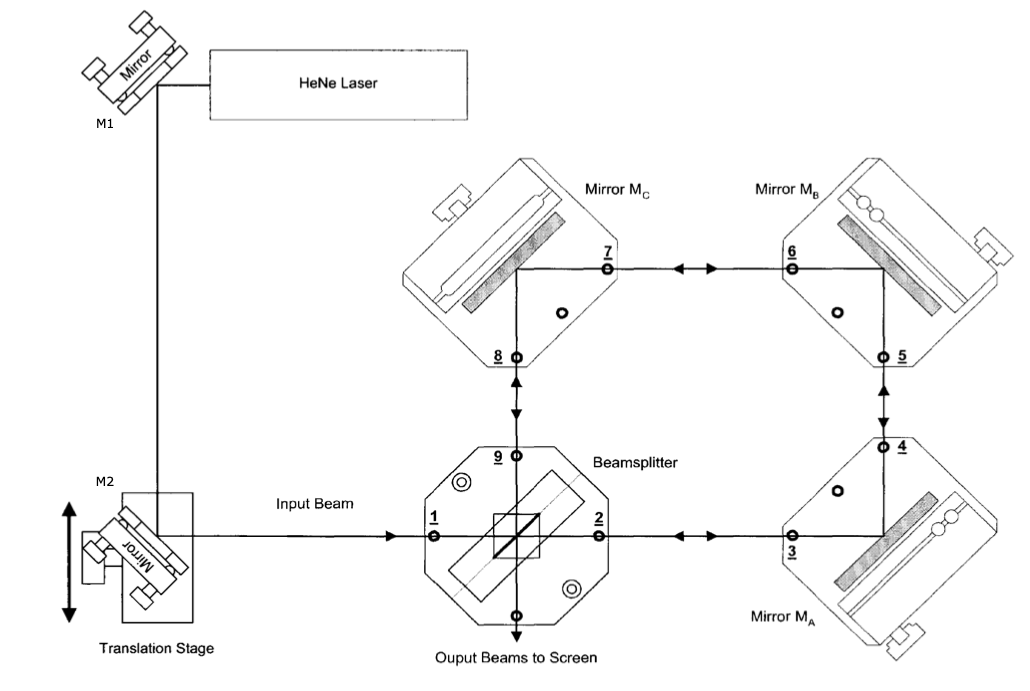
\includegraphics[width=0.8\textwidth]{bilder/Aufbau.png}
    \caption{Schematischer Versuchsaufbau zur Bestimmung der Brechungsindices von Glas und Luft
    mithilfe eines Sagnac-Interferometers \cite{anleitung}.}
    \label{fig:aufbau}
\end{figure} \noindent
Der Aufbau besteht aus einem Helium-Neon-Laser, dessen Laserlicht über die Spiegel M1 und M2 
auf den Strahlteilerwürfel gelenkt wird. Durch diesen wird das einfallende Licht in seinen
horizontal und vertikal linear polarisierten Anteil aufgespalten. Diese durchlaufen den restlichen 
Strahlengang nun in entgegengesetze Richtungen. Der horizontal polarisierte Anteil des Lichtes 
fällt zunächst auf den Spiegel $M_\text{A}$, bevor es auf $M_\text{B}$ und $M_\text{C}$ trifft. 
Der vertikal polarisierte Anteil trifft die Spiegel dementsprechend in umgekehrter Reihenfolge. 
Bevor mithilfe der zwei Dioden eine Intensität gemessen werden kann, treffen beide Teilstrahlen 
erneut auf den Strahlteilerwürfel. Damit eine Interferenzerscheinung messbar ist, ist vor den Dioden
ein weiterer Strahlteilerwürfel positioniert, der um 45° gegenüber dem Strahlengang gekippt ist. \\
Im ersten Versuchsteil wird die Polarisationsrichtung des Laserstrahls bestimmt, die den höchsten
Kontrast aufweist. Dafür wird die Diodenspannung für ein Maximum und ein Minimum bei unterschiedlichen
Polarisationsrichtung bestimmt. Dabei wird in 15°-Schritten gemessen und um das Maximum nochmal
genauer mit 5°-Schritten. Die in diesem Aufgabenteil bestimmte Polarisationsrichtung des Laserstrahls 
mit dem höchsten Kontrast wird für die nachfolgenden Versuchsteile beibehalten. 
Der nächste Versuchsteil dient der Bestimmung der Brechungsindices von Glas und Luft. 
Dafür wird zunächst der Doppelglashalter in den Strahlengang eingesetzt und die Anzahl der Minima und 
Maxima in Abhängigkeit vom Drehwinkels bestimmt. Dafür wird das Oszilloskop und der ANDERE KLOTZ 
genutzt, der die Anzah an Nulldulgängen anzeigt, die dem gesuchten Messwert entsprechen. Dieses
Vorgehen wird 10 mal wiederholt. \\
Um den Brechungsindex vo Luft in Abhängigkeit vom vorherrschenden Druck zu bestimmen, wird eine
Gaszelle in den Strahlengang eingesetzt. Diese wird zunächst evakuiert, um dann geregelt 
Luft zuzuführen. In Abständen von $\SI{50}{\milli\bar}$ wird die Anzahl an Nulldurchgängen notiert 
bis sich der Atmösphärendruck wieder eingestellt hat. Dieses Vorgehen wird vier mal wiederholt.